\documentclass[UTF8,zihao=-4]{ctexart}
\usepackage[a4paper,margin=2.5cm]{geometry}
\usepackage{amsmath, amssymb, amsthm}
\usepackage{bm}
\usepackage{hyperref}
\usepackage{graphicx}
\usepackage{caption}
\usepackage{listings}
\usepackage{xcolor}
\usepackage{float}
\usepackage{booktabs}
\usepackage{longtable}
\usepackage{multirow}
\usepackage{placeins}
\graphicspath{{figures/}}

% 代码样式
\lstdefinestyle{code}{
  basicstyle=\ttfamily\small,
  numbers=left,
  numberstyle=\tiny,
  numbersep=8pt,
  keywordstyle=\color{blue},
  commentstyle=\color{teal!70!black},
  stringstyle=\color{orange!70!black},
  showstringspaces=false,
  breaklines=true,
  frame=single,
  framerule=0.3pt,
  rulecolor=\color{black!15}
}
\lstset{style=code}

\title{模型压缩与蒸馏:剪枝、量化与 TinyLLM 边缘部署}
\author{}
\date{\today}

\begin{document}
\maketitle

\section{剪枝(Pruning)、量化(Quantization)}
\subsection{压缩路线图}
图\ref{fig:compression_landscape_cn} 展示了从全精度 LLM 到轻量化部署模型的典型路径:先通过剪枝降低参数冗余,再通过量化减少数值精度,最后可结合蒸馏形成新的学生模型。
\begin{figure}[H]
  \centering
  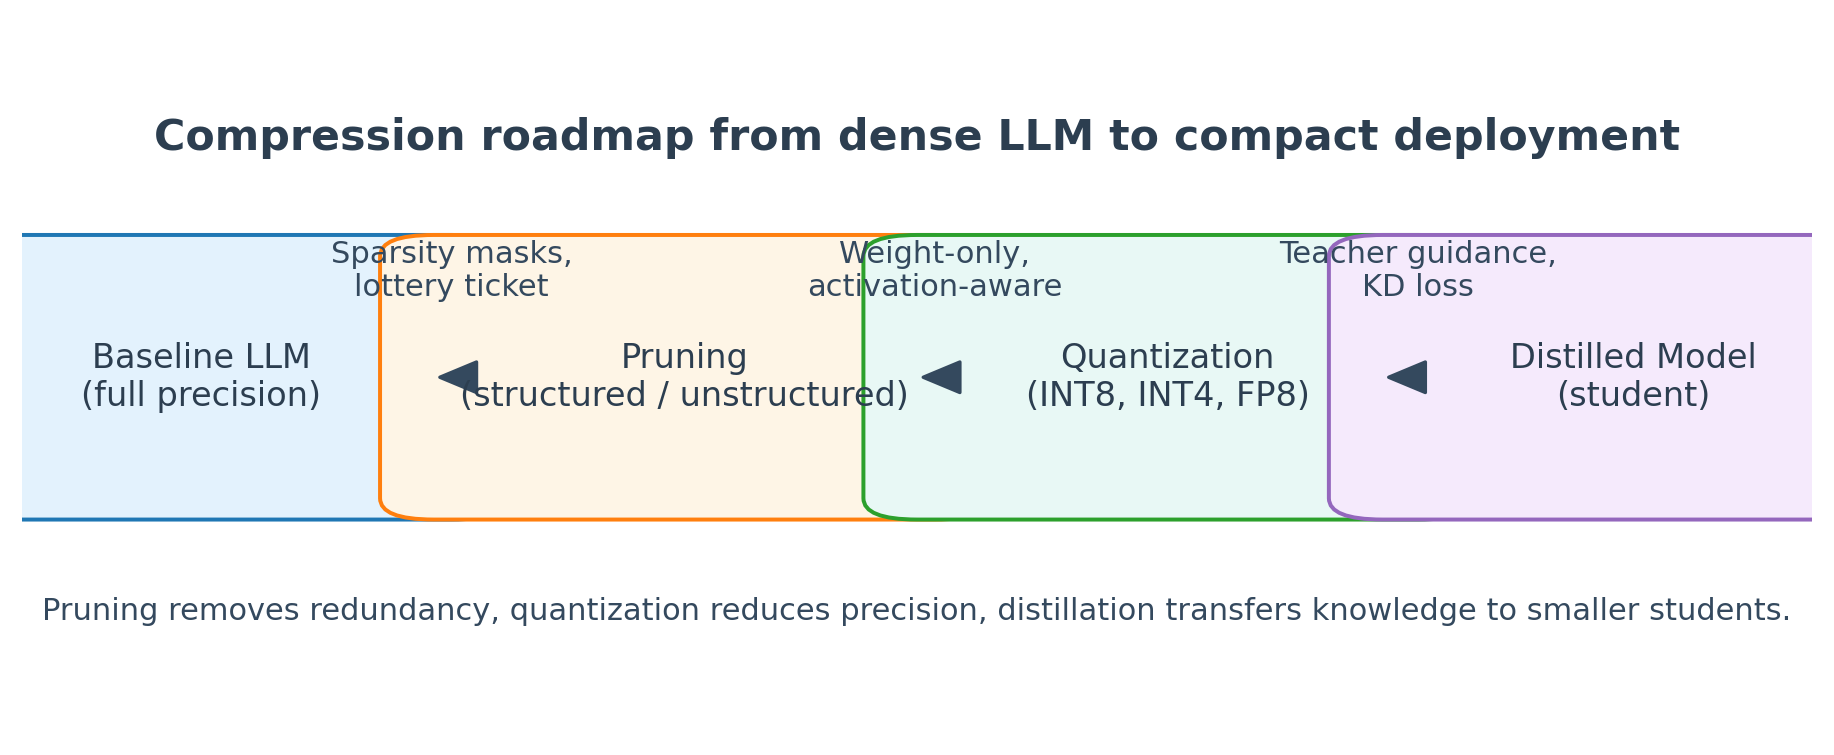
\includegraphics[width=0.9\textwidth]{compression_landscape.png}
  \caption{压缩路线图:剪枝、量化与蒸馏协同减少模型体积与计算量。}
  \label{fig:compression_landscape_cn}
\end{figure}

\subsection{剪枝策略}
\begin{itemize}
  \item \textbf{非结构化剪枝:} 以权重幅值或梯度为指标,将小权重置零;灵活但硬件友好度较低。
  \item \textbf{结构化剪枝:} 去除整列、整头或通道,便于 GPU/CPU 加速;常见于注意力头剪枝、FFN 通道剪枝。
  \item \textbf{动态稀疏:} 训练过程中动态更新稀疏模式(RigL、SNIP),在保持精度的同时提升收敛速度。
  \item \textbf{彩票假说:} 寻找可独立训练的稀疏子网络,为后续微调提供轻量结构。
\end{itemize}

\subsection{量化方法}
\begin{longtable}{p{3cm}p{3cm}p{4cm}p{4cm}}
\toprule
类别 & 位宽 & 特点 & 典型工具 \\
\midrule
动态量化 & INT8 & 推理阶段按批次重新统计量化参数 & PyTorch Dynamic Quantization \\
静态量化 & INT8 & 预先收集校准数据计算 scale/zero-point & TensorRT, ONNX Runtime \\
权重量化 & INT4/INT3 & 仅量化权重,激活保持 FP16 & GPTQ, AWQ \\
激活感知量化 & INT8/INT4 & 同时考虑激活分布,减少误差 & SmoothQuant, AQLM \\
混合精度 & FP8/INT8 & 利用最新硬件(H100、Gaudi2)支持的低精度格式 & TransformerEngine \\
\bottomrule
\end{longtable}

\subsection{量化示例:GPTQ}
\begin{lstlisting}[language=Python,caption={使用 AutoGPTQ 对 LLaMA 权重量化}]
from auto_gptq import AutoGPTQForCausalLM, BaseQuantizeConfig
from transformers import AutoTokenizer

model_name = "meta-llama/Llama-2-7b-hf"
quant_config = BaseQuantizeConfig(
    bits=4,
    group_size=128,
    desc_act=False  # 关闭激活量化
)

model = AutoGPTQForCausalLM.from_pretrained(model_name, quantize_config=quant_config)
tokenizer = AutoTokenizer.from_pretrained(model_name, use_fast=True)

model.quantize(
    examples=["Hello world!", "Quantization reduces memory footprint."],
    batch_size=8,
    use_triton=True,
)

model.save_quantized("llama2-7b-gptq")
tokenizer.save_pretrained("llama2-7b-gptq")
\end{lstlisting}

\section{知识蒸馏(Knowledge Distillation)}
\subsection{蒸馏流程}
知识蒸馏通过教师模型(Teacher)向学生模型(Student)传递知识,常见目标包括:
\begin{itemize}
  \item \textbf{软标签(Soft Targets):} 使用温度系数 $T$ 放大概率分布,学生最小化 KL 散度。
  \item \textbf{中间层对齐:} 蒸馏注意力、隐藏状态、梯度统计等中间特征,增强学生表达力。
  \item \textbf{任务蒸馏:} 将教师模型在真实任务上的输出作为监督信号(SFT+KD)。
\end{itemize}

\subsection{损失函数设计}
综合蒸馏损失可写为:
\begin{equation}
\mathcal{L} = \alpha \cdot \mathcal{L}_{\text{KD}}(p_s, p_t) + \beta \cdot \mathcal{L}_{\text{task}}(y_s, y_{\text{true}}) + \gamma \cdot \mathcal{L}_{\text{feature}}(h_s, h_t),
\end{equation}
其中 $p_s$、$p_t$ 分别为学生与教师的 softmax 输出,$h$ 代表中间特征,$\alpha,\beta,\gamma$ 控制权重。

\subsection{蒸馏案例}
\begin{itemize}
  \item \textbf{TinyLlama:} 基于 3 亿参数的小模型,通过蒸馏大模型指令数据获得接近 7B 模型的能力。
  \item \textbf{MiniLM:} 利用深度自注意力蒸馏,让 384 维模型达到 BERT-base 的效果。
  \item \textbf{LLaDA:} 在多语言任务中将多模态知识蒸馏到紧凑模型。
\end{itemize}

\subsection{蒸馏伪代码}
\begin{lstlisting}[language=Python,caption={Teacher-Student 蒸馏训练循环简例}]
for batch in dataloader:
    with torch.no_grad():
        teacher_logits, teacher_hidden = teacher(**batch, output_hidden_states=True)

    student_logits, student_hidden = student(**batch, output_hidden_states=True)

    loss_kd = kl_divergence(
        F.log_softmax(student_logits / T, dim=-1),
        F.softmax(teacher_logits / T, dim=-1)
    ) * (T * T)

    loss_task = cross_entropy(student_logits, batch["labels"])
    loss_hidden = mse_loss(student_hidden[-1], projector(teacher_hidden[-1]))

    loss = alpha * loss_kd + beta * loss_task + gamma * loss_hidden
    loss.backward()
    optimizer.step()
    optimizer.zero_grad()
\end{lstlisting}

\section{TinyLLM 与边缘设备部署}
\subsection{部署栈概览}
图\ref{fig:tinyllm_edge_stack_cn} 描述了 TinyLLM 在边缘侧部署的核心组件:上游压缩流水线产生量化模型,TinyLLM Runtime 利用特定硬件内核执行,遥测与编排层实现反馈闭环。
\begin{figure}[H]
  \centering
  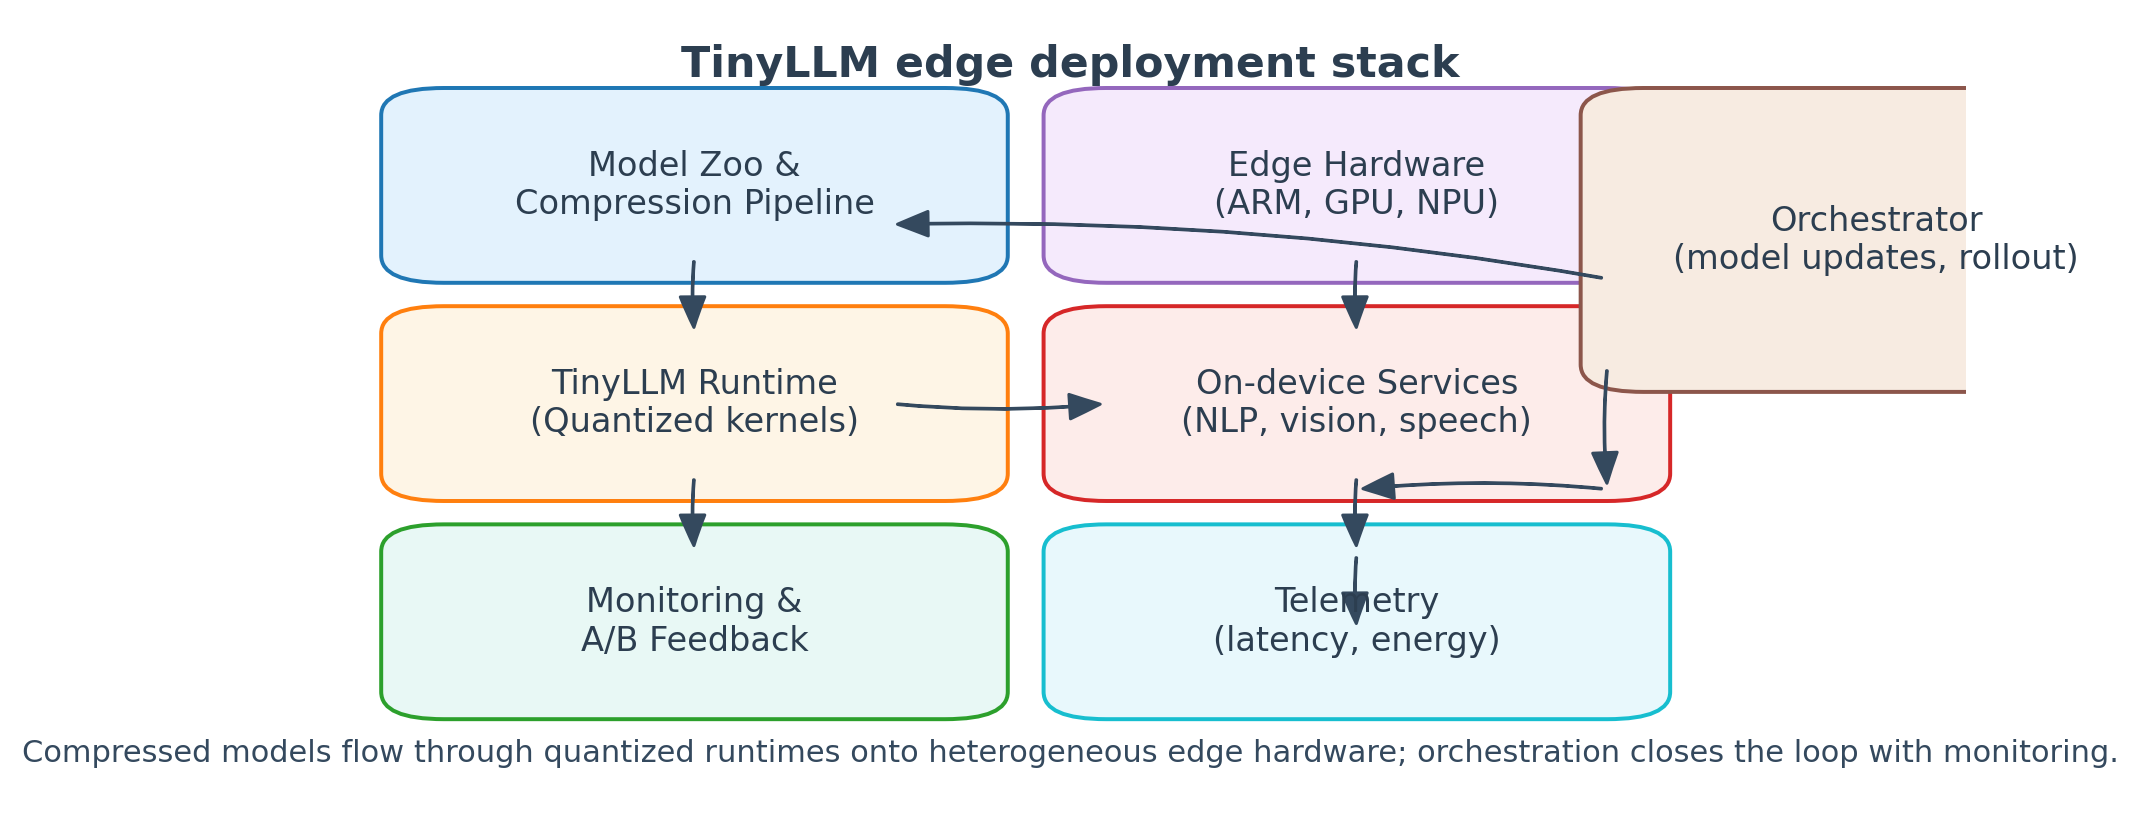
\includegraphics[width=0.9\textwidth]{tinyllm_edge_stack.png}
\caption{TinyLLM 边缘部署栈:压缩流水线、量化运行时、异构硬件与编排治理。}
  \label{fig:tinyllm_edge_stack_cn}
\end{figure}

\subsection{TinyLLM Runtime}
\begin{itemize}
  \item \textbf{内核优化:} 针对 INT4/INT8 张量核、张量切片、流水线并行进行优化;
  \item \textbf{内存管理:} 采用静态内存池、KV Cache 压缩(grouped-query attention);
  \item \textbf{调度策略:} 支持多租户、批处理、自适应延迟控制。
\end{itemize}

\subsection{边缘硬件适配}
\begin{longtable}{p{3cm}p{3cm}p{4cm}p{4cm}}
\toprule
硬件 & 精度支持 & 典型场景 & 工具栈 \\
\midrule
ARM CPU (Neon) & INT8/INT4 & 移动端对话、离线助手 & MNN, NCNN, llama.cpp \\
NVIDIA Jetson & FP16/INT8 & 机器人、工业检测 & TensorRT, FasterTransformer \\
Apple Neural Engine & 8-bit & iOS 应用内推理 & Core ML, Metal Performance Shaders \\
定制 NPU & INT4/INT2 & 智能家居、车载系统 & ONNX Runtime EP, TVM \\
\bottomrule
\end{longtable}

\subsection{部署流水线}
\begin{enumerate}
  \item \textbf{模型准备:} 对基础模型执行剪枝 + 量化 + 蒸馏形成学生模型;
  \item \textbf{格式转换:} 导出为 ONNX、TensorRT engine、Core ML、GGUF 等;
  \item \textbf{运行时集成:} 嵌入 TinyLLM Runtime 或各类推理框架(MNN、llama.cpp);
  \item \textbf{监控闭环:} 收集延迟、能耗、质量指标,回传云端重新蒸馏或更新模型。
\end{enumerate}

\subsection{部署脚本示例}
\begin{lstlisting}[language=Python,caption={使用 llama.cpp 推理量化模型}]
import subprocess
import pathlib

MODEL_PATH = pathlib.Path("models/tinyllm-q4_0.gguf")
PROMPT = "Summarize the daily production report in Chinese."

cmd = [
    "./main",
    "-m", str(MODEL_PATH),
    "-p", PROMPT,
    "-n", "128",
    "--temp", "0.8",
    "--batch-size", "32",
    "--threads", "8"
]

result = subprocess.run(cmd, capture_output=True, text=True, check=True)
print(result.stdout)
\end{lstlisting}

\section*{实践建议}
\begin{itemize}
  \item 将剪枝、量化、蒸馏视为组合拳,先评估精度敏感度再选择策略;
  \item 对压缩模型进行系统化评测:困惑度、下游任务、延迟、能耗、安全性;
  \item 建立持续学习与反馈回路,利用边缘日志改进蒸馏数据与模型版本;
  \item 注重安全与隐私:在边缘端启用本地推理可减少数据外泄风险,但仍需加密存储和访问控制。
\end{itemize}

\section*{参考文献}
\begin{itemize}
  \item Frantar et al. ``GPTQ: Accurate Post-Training Quantization for Generative Pre-trained Transformers.'' NeurIPS, 2022.
  \item Dettmers et al. ``QLoRA: Efficient Finetuning of Quantized LLMs.'' NeurIPS, 2023.
  \item Sanh et al. ``DistilBERT, a distilled version of BERT.'' NeurIPS, 2019.
  \item Zhang et al. ``TinyLlama: Tiny Language Models for Edge AI.'' arXiv, 2024.
  \item Li et al. ``AWQ: Activation-aware Weight Quantization for LLM Compression and Acceleration.'' arXiv, 2023.
\end{itemize}

\end{document}

